\documentclass[10pt,twocolumns,letterpaper]{article}
%---------------------Paquetes-----------------------------------------------%
\usepackage[spanish]{babel}
\usepackage[latin1,utf8]{inputenc}
\usepackage{amssymb,amsmath} %Lenguaje matemático %amsmath, el de las integrales
\usepackage{verbatim} %Escribir código
\usepackage{bm}
\usepackage{graphics,graphicx,xcolor}
\usepackage{subfigure} % subfiguras
\usepackage{multirow}
\usepackage{caption}
%\usepackage{subcaption}
\usepackage{subfig}
%% Sets page size and margins
\usepackage[a4paper,top=2cm,bottom=2cm,left=2cm,right=2cm,marginparwidth=1.75cm]{geometry}

\usepackage{multicol}
\usepackage{longtable} % para tablas largas
%---------------------Título-------------------------------------------------%
\title{
		\usefont{OT1}{bch}{b}{n}
		\normalfont \normalsize \textsc{Laboratorio de Física moderna II.} \\ [10pt]
		\Large Decaimiento Beta del $^{22}Na$ por Deflexión Magnética.\\  Carlos Andrés Rodallega \& Brayan Eraso}
\date{}
\selectlanguage{spanish}
%---------------------------------Documento---------------------------------%
\begin{document}
\twocolumn[
\begin{@twocolumnfalse}
\maketitle
\vspace*{-1.8cm}
\begin{abstract}
Cuando sobre la radiación beta se aplica un campo magnético perpendicular a la fuente de emisión de radiación, la radiación presenta un deflexión que puede ser descrita como un arco de circunferencia. Se estudia esta deflexión en el proceso de decaimiento del isótopo del Sodio $^{22}Na$ en función del campo magnético aplicado, para ello, se utilizó una sonda Hall, un par de imanes de neodimio y un detector Geiger-Müller. El análisis de los datos obtenidos se realizó según la estadística de Fermi-Dirac y se utilizó el modelo de Kuri-Fermi para los gases, en base a este modelo se pudo estimar que la energía cinética máxima asociada al proceso de decaimiento ($\beta$) del Sodio, la cual fue de $E_0 = 0.72\pm 0.02 MeV$.. \\ 
\\
\textbf{Palabras clave}: \textit{Radiación Beta, Deflexión Magnética, Energía máxima de la radiación Beta.}
\vspace*{0.2cm}
\end{abstract}
\end{@twocolumnfalse}
]

\section{Introducción}
El decaimiento radiactivo Beta ($\beta$) es la emisión espontánea de un electrón o un positrón de alta energía y alta velocidad emitido por un núcleo atómico. La siguiente relación nuestra el proceso de desintegración Beta negativo $\beta^{+}$ (Emisión de positrones):
\begin{equation} \label{eqn_1}
    P \longrightarrow N+e^{+}+{v}_e
\end{equation}
Siendo ${v}_{e}$ el neutrino correspondiente necesario para satisfacer el principio de conservación del número leptónico.\\ \\  El estudio del comportamiento de la radiación Beta es esencial en la física nuclear debido a que nos ayuda comprender el fenómeno de la radiactividad y sus aplicaciones son esenciales en diversos campos de la física e incluso también en la medicina. \\ \\
Como parte de estudio del comportamiento de la radiación Beta se estudia la deflexión magnética de las partículas emitidas en un decaimiento Beta. Se sabe que en un decaimiento Beta surgen electrones o positrones como resultado de la desintegración radiactiva, dichas componentes pueden ser deflectadas por un campo magnético debido a que son partículas cargadas. \\ \\ 
Para esto se realiza una práctica donde se podrá estudiar la deflexión de partículas radiactivas, partículas de Sodio-22 ($^{22}Na$) en función de la magnitud de un campo magnético aplicado en la dirección perpendicular a su movimiento, esto hará que las partículas cargadas sufran una deflexión debido a que hay una fuerza actuando sobre ellos (Fuerza de Lorentz), posteriormente se podrán analizar los datos obtenidos para establecer la energía cinética de las partículas en función del campo magnético aplicado, lo que nos permitirá obtener una relación directa entre el número de partículas radiactivas deflectadas y la energía cinética de las mismas.

\section{Marco Teórico}
Con base en lo dado en la Guía de laboratorio de física moderna II \cite{b3}, cuando las partículas $\beta$ de una muestra radiactiva se colocan bajo la influencia de un campo magnético transversal, las partículas serán medidas en un detector Geiger-Müller después de haber descrito un arco de circunferencia cuya curvatura es:
\begin{equation}\label{eqn_2}
    r=\frac{R}{tan(\frac{\theta}{2})}
\end{equation}
Siendo R el radio de los polos de los imanes utilizados para crear el campo magnético y $\theta$ el ángulo entre el detector y el emisor.\\
Vemos que la cantidad de movimiento de las partículas está relacionada con la fuerza de Lorentz (\ref{eqn_3}) y la energía cinética de las partículas se expresa con el formalismo relativista (debido al tamaño de las masas) dado por (\ref{eqn_3})
\begin{equation}\label{eqn_3}
   evB=\frac{mv^2}{r}
\end{equation}
\begin{equation}\label{eqn_4}
    E= p^2 c^2 + m^2 c^4 
\end{equation}
Por lo cual, podemos expresar la energía cinética (\ref{eqn_4}) y remplazar toda la información anterior (\ref{eqn_5})
\begin{gather}
    E = E_k + m_0 c^2 \longrightarrow E_k = E - m_0 c^2 \label{eqn_5}\\
   E_k = m_0 c^2\left(\sqrt{\left(\frac{e B R}{m_0 c tan^\frac{\theta}{2}}\right)^2+1}-1\right) \label{eqn_6}
\end{gather}
Así, fijando en nuestro experimento $B$ y $\theta$ es posible obtener la energía cinética $E_k$. \\ \\
Para el análisis del espectro de emisión de las partículas Betas, se usa el carácter fermiónico de las partículas vistas en la relación(\ref{eqn_1}), para esto se debe utilizar la estadística de Fermi-Dirac y se utiliza el modelo de Kurie y Fermi para los gases, así se obtiene una relación directa (\ref{eqn_6}) entre el número de cuentas por unidad de tiempo y la energía cinética.
\begin{equation}\label{eqn_7}
    \sqrt{\frac{N(t)}{p^2_e}} \propto (E_0 - E_k)
\end{equation}
\section{Metodología}
Se genera un campo magnético constante con la ayuda de dos imanes permanentes de neodimio, dichos imanes se encuentran separados a una distancia variable que permite variar la magnitud del campo magnético generado. Se ubica una sonda Hall entre los imanes y se ubican de manera perpendicular entre sí el detector Geiger-Müller y la fuente de partículas radiactivas ($\beta$). En la figura(\ref{fig:1}) se puede apreciar lo mencionado, de izquierda a derecha se ubica el teslametro, el detector, la sonda hall, los imanes y la fuente radiactiva.
\begin{figure}[h!]
    \centering
    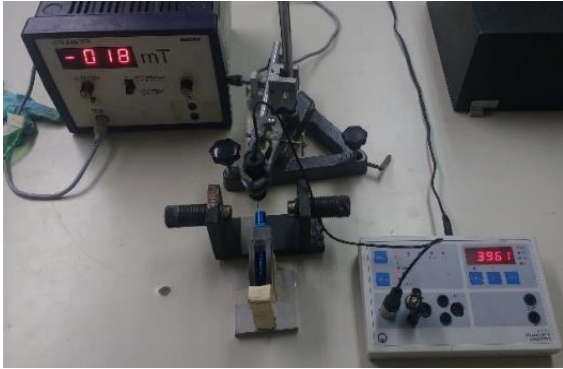
\includegraphics[scale=0.5]{Montaje_Exp.png}
    \caption{Montaje experimental y Equipos utilizados para estudiar la deflexión beta.}
    \label{fig:1}
\end{figure} \\
Después de haber realizado el montaje experimental, se mide el campo magnético máximo y mínimo que se puede generar al variar la distancia entre los imanes, se realiza su diferencia, se divide por 30 y se encuentra él $\Delta B$, que es la magnitud de campo magnético que se va a variar entre cada medición.\\ \\
El detector Geiger-Müller se programa para medir el número de cuentas realizadas en 10 segundos y se realizan 3 tomas de datos por cada proceso de medición, esto para trabajar con un promedio.\\ \\
En el proceso de medición, se coloca el campo magnético mínimo otorgado por los imanes y se mide el número de cuentas dadas por el detector en función del campo magnético, realizando este proceso 30 veces y aumentando el campo magnético en la magnitud $\Delta B$ mencionada. 
\section{Resultados}
Como primer resultado del proceso de medición se obtienen los datos por la figura (\ref{fig:2}), posteriormente, al realizar el tratamiento de datos según las ecuaciones (\ref{eqn_6}) y (\ref{eqn_7}), se obtienen los datos ilustrados en las figuras (\ref{fig:3}) y (\ref{fig:4}).\\ \\
Se puede apreciar que los datos dados por la figura (\ref{fig:4}) presentan un ajuste lineal, esto se realiza con el objetivo de obtener la energía máxima $E_0$ del decaimiento $\beta$, que es el punto de corte de la recta con el eje de la energía en la Curva Kuri-Fermi. Dicho resultado obtenido fue:

$$ E_0 = 0.72\pm 0.02 MeV$$
\begin{figure}[h]
    \centering
    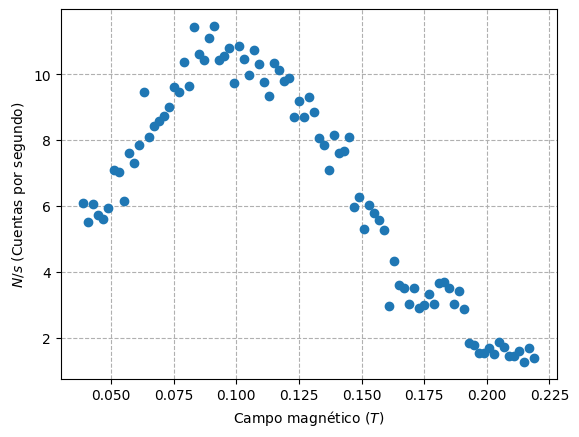
\includegraphics[scale=0.6]{Datos tomados.png}
    \caption{Cuentas radiactivas por unidad de tiempo $(N/s)$ en función del campo magnético aplicado.}
    \label{fig:2}
\end{figure} 

\begin{figure}[h!]
    \centering
    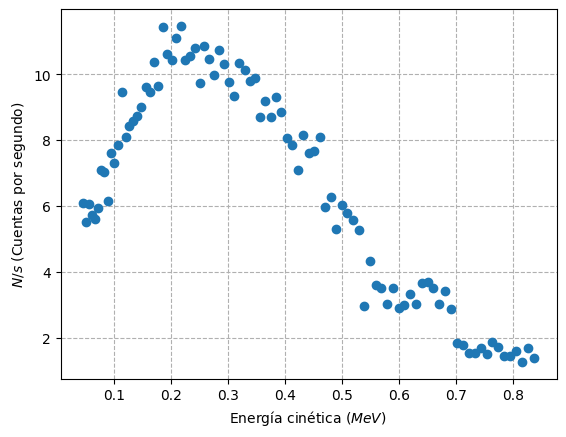
\includegraphics[scale=0.6]{Imagen corregida.png}
    \caption{Cuentas radiactivas por unidad de tiempo $(N/s)$ en función de la energía cinética de las partículas.}
    \label{fig:3}
\end{figure}

\begin{figure}[h!]
    \centering
    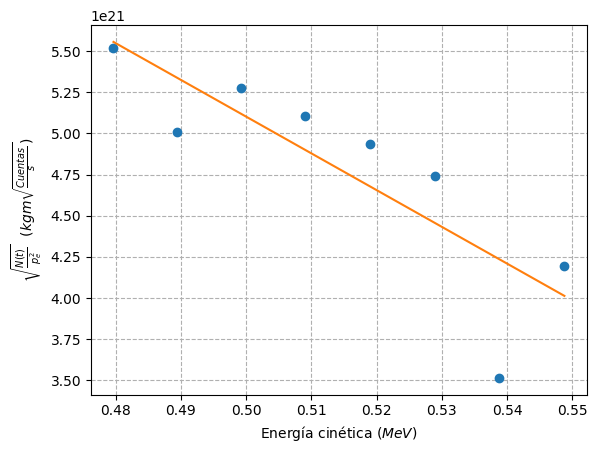
\includegraphics[scale=0.55]{Ajuste.png}
    \caption{Gráfica de $\sqrt{\frac{N(t)}{p^2_e}}$ en función de la energía cinética $E_k$, con la extrapolación de la mejor recta de los datos de bajada.}
    \label{fig:4}
\end{figure}
\section*{Conclusiones}
Desde la parte experimental se evidenció directamente el fenómeno de la deflexión magnética de los electrones o positrones involucrados en un decaimiento $\beta$, a su vez, se encontró que el número de cuentas en función del campo magnético aplicado tiene un crecimiento hasta llegar a un máximo desde el cual empieza a disminuir, se asemeja a un comportamiento Gaussiano. Además, se observó experimentalmente que las partículas involucradas en este decaimiento son partículas cargadas debido al comportamiento mostrado.  \\ \\
Los resultados obtenidos para la energía cinética máxima de las partículas involucradas en el decaimiento beta fue de  $E_0 = 0.72\pm 0.02 MeV$, que es un resultado que difiere bastante a lo presentado en la literatura, que es de aproximadamente $E_0 = 0.54 \:  MeV$, hay muchas causas en la gran diferencia entre los resultados y más adelante las trataremos. \\ \\
Al igual que la práctica de deflexión electromagnética por estroncio, se encuentra un valor para la energía $E_0$, en este caso vemos que el sodio presenta una energía cinética debido a la deflexión de partículas de radiación beta menor a la energía dada por la deflexión de partículas de estroncio, esto es debido a que la masa de ambas partículas son diferentes, siendo la masa del sodio mucho menor, lo que implica que la energía cinética adquirida durante la deflexión es menor. \\ \\
El modelo implementado para realizar el análisis, es decir, el modelo de Kuri-Fermi, es válido en ciertos intervalos de energía, que es donde realizamos el ajuste lineal para obtener la energía máxima del decaimiento. A pesar de obtener un valor de energía máxima que difiere mucho por el reportado en la bibliografía, esto no quiere decir que el modelo tenga alguna inconsistencia, esto debido a que la gran impresión de este experimento se debe a factores experimentales qué teóricos.  \\ \\
%Las posibles causas de error experimentales puede ser que no se consideró la radiación del fondo en un lugar de laboratorio que contiene muchas muestras radiactivas realizando mediciones entre sí, además el hecho de contar con imanes de neodimio y no electroimanes, genera que los imanes se desgasten con el tiempo y no generen un campo magnético lo suficientemente grande para poder deflectar las partículas radiactivas.\\ \\
Como recomendación, para evitar todos estos posibles errores se recomienda medir el promedio de la radiación de fondo en el lugar que se está trabajando y realizar mediciones con electro imanes, posteriormente se recomienda ser muy cuidadosos en el rango de energía en el cual se realizará el análisis bajo el modelo de Kuri-Fermi, debido a que este no es aplicable en todo el espectro de energía que obtengamos.
\begin{thebibliography}{99}
\bibitem[1]{b1} Mera, E. (2015). Experimento: Radiación. Universidad Tecnológica Metropolitana de Chile.

\bibitem[2]{b2} Ram, N., Sundara Rao, I.S. \& Mehta, M.K. Mass absorption coefficients and range of beta particles in Be, Al, Cu, Ag and Pb. Pramana - J. Phys. 18, 121–126 (1982). 
\bibitem[3]{b3} Miranda, E.B., Zuleta, C.A y Bastidas J. P ., Guías de Laboratorio FÍSICA MODERNA II. Facultad de Ciencias Naturales y Exactas. Departamento de Física. Universidad del Valle. 10-14 (2023).
\end{thebibliography} 



\end{document}

